\subsubsection{Signup/Login Sequence Diagram}

This sequence diagram points out the steps to make a proper signup and to correctly login to Travlendar+ as a specific
user. As you can see, there are three main phases, fulfilling the registration form, verifying the user email and logging in. 
In order to mark up the differences between  registered and  unregistered customers, we called them respectively 'user' and 'guest'. 
Clearly, the email verification leads to an automatic login, thus the system redirects the user to his personal page. This also explain why we inserted logout before the login step. 

\begin{figure}[htp]
	
	\centering
	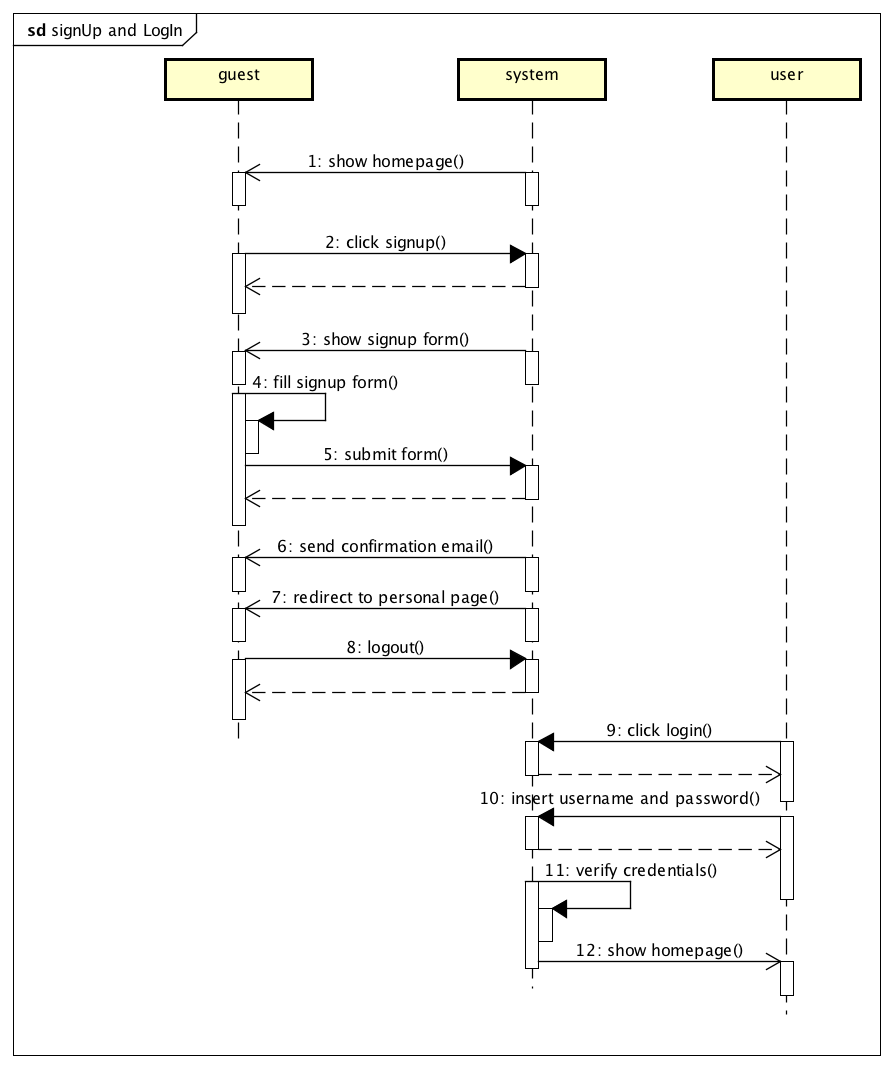
\includegraphics[width=\textwidth]{sequencediagrams/signup-logIn}
	\caption{The sequence diagram about Signup and Login operations.}
	\label{fig:signup-login} 

\end{figure}
\newpage

\subsubsection{Meeting Creation Sequence Diagram}

This sequence diagram explains how to create a meeting, assuming that the operation is accomplished properly.
Oppositely,in case of failures such as trying to insert a duplicate meeting, Travlendar+ prevents the appointment registration. 
As the chart shows, when a user selects a date on the calendar, the system provides him a meeting form, where he can insert all the required information. Then, the app enters in an intense computational phase. In addition to the local operations such as verifying overlappings and analyzing preferences, during this step Travlendar+ also interacts with external systems. 
We labeled them as 'service providers' referring for example to the public transports server, a forecast agency infrastructure, sharing services systems etc, and we suppose the related events to be database queries. 
The entire process ends with the registration of the event into the system and a positive notification to the user. 

\begin{figure}[htp]
	
	\centering
	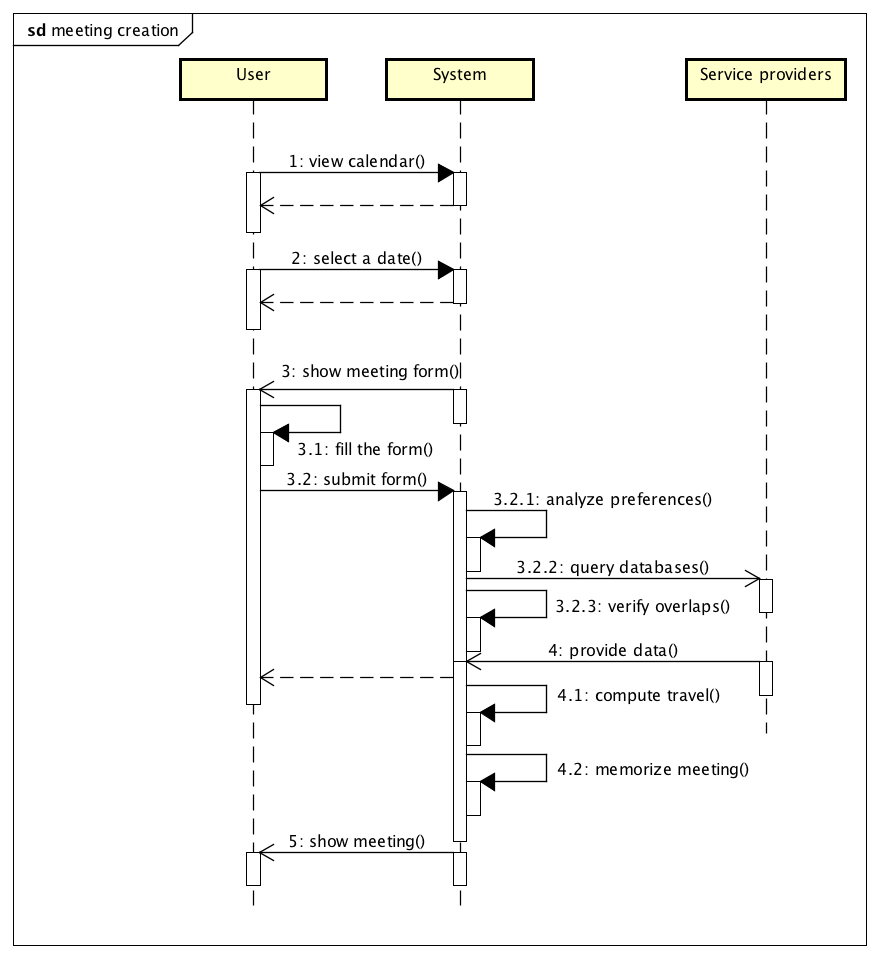
\includegraphics[width=\textwidth]{sequencediagrams/meetingcreation}
	\caption{The sequence diagram about the process flow of a meeting creation.}
	\label{fig:meetingcreation}
		
\end{figure}
\newpage

\subsubsection{Warnings Solving Sequence Diagram}

The last two sequence diagrams refer to the user reaction against the generation of a warning by the system. 
In order to model correctly the two possibile user choices, we have done two diagrams, one for each possibility. 
The first and simple chart explains what happens if the user decides to ignore a warning, that is just the deletion of the notification, because we assume his specific intention not to consider it. 
The second diagram, quite more complex, regards the warning resolution through an event rescheduling made by the user. For this reason, Travlendar+ allows to directly go from the warning to the conflictual meetings, in order to modify them. 
Obviously, considering that a conflict, same as a warning, can involve from two up to a huge number of appointments, it is clear that the operation number 5 could be done for more than just one meeting involved in the conflict. 

\begin{figure}[htp]
	\centering
	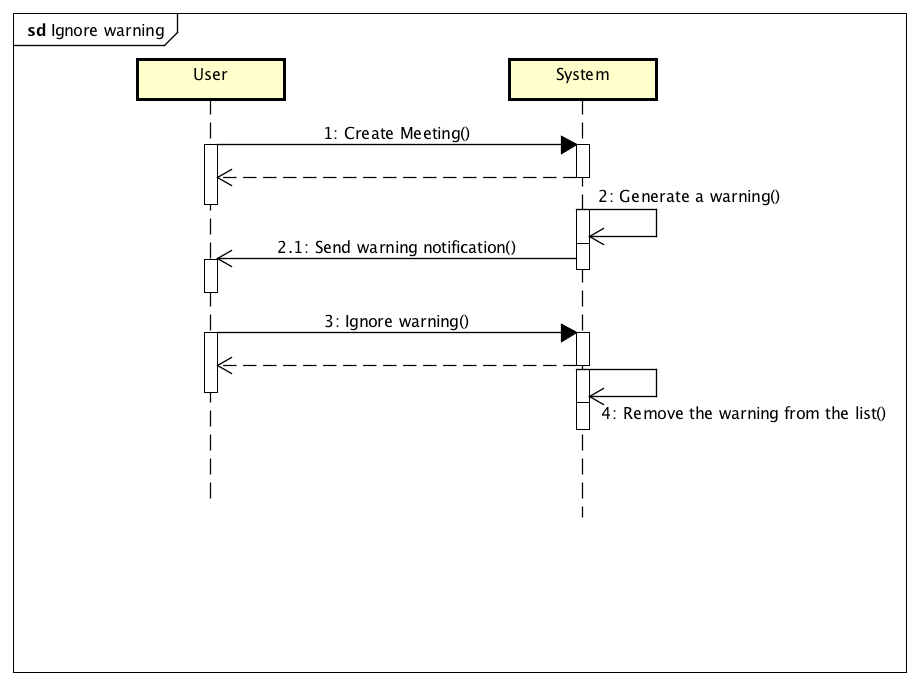
\includegraphics[width=\textwidth]{sequencediagrams/Ignorewarning}
	\caption{The sequence diagram that shows the steps to ignore a warning.}
	\label{fig:ignorewarning}
\end{figure}

\begin{figure}[htp]

	\centering
	\includegraphics[width=\textwidth]{"sequencediagrams/ warningresolution"}
	\caption{the sequence diagram that shows how to solve a warning.}
	\label{fig:-warningresolution}
	\begin{center}

	\end{center}
\end{figure}
\newpage


